
\documentclass[ ngerman, fontsize= 10pt, headings=big, titlepage=true]{beamer}

\usepackage{babel}
\usepackage[utf8]{inputenc}
\usepackage[T1]{fontenc}

%\usepackage{lmodern, microtype}
\usepackage{csquotes}
\usepackage{hyperref}
\usepackage{enumerate}

%Tablellen:
\usepackage{multirow}
\usepackage{caption}
\usepackage{booktabs}
\usepackage{rotating}
\usepackage{hhline,float}

%Mathematik
\usepackage{amsmath}
\usepackage{amsfonts}
\usepackage{amssymb}
\usepackage{mathtools}
\usepackage{bbm}
\usepackage{color}
%R-Code
\usepackage{xcolor}

\usetheme{Dresden}
\usecolortheme{spruce}

\title{Grundlagen der Versuchsplanung-Experiment 1}
\subtitle{Längenschätzen}
\author{Kaya Maria Bayer \and Ketevan Gurtskaia \and Alicia Hemmersbach \and Danuscha Große-Hering}
\date{07.Juni 2021}
\begin{document}
\begin{frame}[plain]
    \maketitle
\end{frame}

\begin{frame}{Inhaltsverzeichnis}
	\tableofcontents
\end{frame}

\section{Einleitung}
\begin{frame}{Einleitung}
\end{frame}

\section{Problemstellung und Versuchsbedingungen}
\begin{frame}{Problemstellung und Versuchsbedingungen}
	
\end{frame}

\section{Analyse des Problems}
\begin{frame}{Analyse des Problems}
	Inhalt...
\end{frame}

\section{Modell, Hypothesen und statistische Auswertungsmethoden}
\begin{frame}{Modell, Hypothesen und statistische Auswertungsmethoden}
	Inhalt...
\end{frame}

\section{Versuchsplanung (1/4)}
\begin{frame}{Versuchsplanung}
	\textbf{1. Grafische Bestimmung der minimalen Stichprobengröße}\\
	$\alpha =0.05$, $\beta = 0.95$ und $\delta =0.5$\\
	 Betrachte die Stichprobengröße n $\in [1,28]$
	 
	\begin{center}
		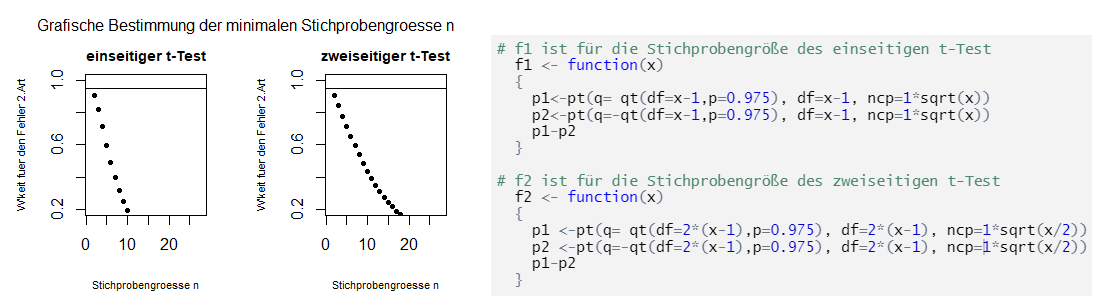
\includegraphics[scale=0.4]{Stichprobengröße.png}
	\end{center}

	$\Rightarrow n > 0$
\end{frame}

\begin{frame}{Versuchsplan (2/4)}
	
	
	\begin{itemize}
		\item Faktor: Reihenfolge der Länge (2 Stufen)
		\item Block: Papiergröße (2 Stufen), Stiftgröße(2 Stufen)	
		\item balanzierten Versuchsplan\\
		 $\Rightarrow n = S_{Faktor} \cdot S_{Block\ A} \cdot  S_{Block\ B} \cdot k =2 \cdot 2\cdot 2\cdot k = 8\cdot k$ \\
		 mit k $\in \mathbb{N}_+$
		
		\item mögliche Probanden =28 $\Rightarrow$ k = 3 $\Rightarrow$ n=24 (Zufällig)
		\item Fehler 2.Art mit n=24 : ca.0.35 (einseitiger t-Test), ca.0.6 (zweiseitiger t-Test)
		
		
	\end{itemize}
	
\end{frame}
\begin{frame}{Versuchsplanung (3/4)}
	
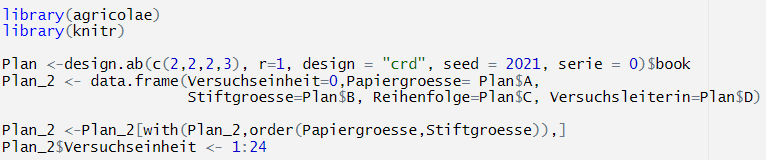
\includegraphics[scale=0.7]{Code_Versuchsplan.png}

{\small
\begin{table}[hb]
	\caption{Versuchsplan 1.Hälfte}
	\centering
	\begin{tabular}[b]{l||l|l|l|l|l|l|l|l|l|l|l|l}
		\hline
		Einheit & 1 & 2 & 3 & 4 & 5 & 6 & 7 & 8 & 9 & 10 & 11 & 12\\
		\hhline{=============}
		Block A & 1 & 1 & 1 & 1 & 1 & 1 & 1 & 1 & 1 & 1 & 1 & 1\\
		\hline
		Block B & 1 & 1 & 1 & 1 & 1 & 1 & 2 & 2 & 2 & 2 & 2 & 2\\
		\hline
		Faktor & 2 & 2 & 2 & 1 & 1 & 1 & 2 & 2 & 1 & 1 & 1 & 2\\
		\hhline{=============}
		{\tiny Versuchsleiterin} & 1 & 3 & 2 & 3 & 1 & 2 & 2 & 3 & 2 & 1 & 3 & 1\\
		\hline
	\end{tabular}
\end{table}}

\end{frame}
\begin{frame}{Versuchsplanung (4/4)}
	
{\small
\begin{table}[hb]
	\caption{Versuchsplan 2.Hälfte}
	\centering
	\begin{tabular}[b]{l||l|l|l|l|l|l|l|l|l|l|l|l}
		\hline
		Einheit & 13 & 14 & 15 & 16 & 17 & 18 & 19 & 20 & 21 & 22 & 23 & 24\\
		\hhline{=============}
		Block A & 2 & 2 & 2 & 2 & 2 & 2 & 2 & 2 & 2 & 2 & 2 & 2\\
		\hline
		Block B & 1 & 1 & 1 & 1 & 1 & 1 & 2 & 2 & 2 & 2 & 2 & 2\\
		\hline
		Faktor & 2 & 1 & 1 & 2 & 2 & 1 & 2 & 1 & 1 & 1 & 2 & 2\\
		\hhline{=============}
		{\tiny Versuchsleiterin} & 3 & 2 & 3 & 1 & 2 & 1 & 2 & 2 & 3 & 1 & 1 & 3\\
		\hline
	\end{tabular}
\end{table}}

\begin{itemize}
	\item Block A $\hat{=}$ Papiergröße mit zwei Stufen: 1:= A4 und 2:= A3  
	\item Block B $\hat{=}$ Stiftgröße auch mit zwei Stufen:  1:= 0.5mm und 2:=2mm 
	\item Faktor $\hat{=}$ Reihenfolge der Längen: 1:= zuerst 5cm und 2:= zuerst 20cm
\end{itemize}

\end{frame}



\section{Literaturverzeichnis}
\begin{frame}{Literaturverzeichnis}
	Inhalt...
\end{frame}

\end{document}
